\chapter{Aplicaci\'on de la t\'ecnica de simulaci\'on Monte Carlo}
% \markboth{Intr. proc. im\'agenes radiol\'ogicas \'ambito m\'edico \ \textbf{M\'ODULO VII}}{ESPECIALIDAD III \ \textbf{M\'ODULO VII}}
\label{CapVII}

El \textit{Cap\'itulo} \ref{CapVII} presenta algunos ejemplos sencillos, pero ilustrativos del modo en que puede aplicarse y aprovecharse la 
t\'ecnica Monte Carlo con fines de c\'omputo num\'erico. se muestran algunas aplicaciones gen\'ericas, como estimaci\'on de n\'umeros y 
c\'alculo de integrales definidas. Por \'ultimo se realiza un ejemplo de aplicaci\'on simple respecto de c\'omo emplear el m\'etodo Monte 
Carlo para modelar el transporte de radiaci\'on.

\section{Introducci\'on}
% \markboth{Intr. proc. im\'agenes radiol\'ogicas \'ambito m\'edico \ \textbf{M\'ODULO VII}}{ESPECIALIDAD III \ \textbf{M\'ODULO VII}}
\label{CapVII_1}

Tal como se enunci\'o en secciones precedentes, existe una amplia variedad de problemas asociados al modelado del transporte de radiaci\'on,
y que de hecho se presentan en la pr\'actica en muy diversos \'ambitos, que carecen de soluci\'on dentro del campo anal\'itico, limitando 
el uso de ``matem\'atica pura'' para la resoluci\'on de los mismos. 
%

Este es el caso, por ejemplo, de la resoluci\'on de algunas ecuaciones \'integro-diferenciales. En particular, existen varios teoremas que 
demuestran la gran limitaci\'on de los m\'etodos anal\'iticos para la resoluci\'on directa de la ecuaci\'on de transporte de Boltzmann, 
representada por la expresi\'on \ref{EqX}. De hecho, se conoce como resultado de teoremas que s\'olo puede resolverse la ecuaci\'on de 
transporte de Boltzmann para una cantidad muy acotada de situaciones, involucrando condiciones iniciales y de contorno que resultan muy poco 
realistas en casos de aplicaci\'on concreto de problemas f\'isicos.
%

Por tanto, se propone un m\'etodo alternativo para encontrar soluciones a la ecuaci\'on \ref{EqX}, para lo cual se considerar\'a la 
re-escritura del problema en modo particular para posteriormente aplicar un procedimiento que consiste, b\'asicamente, en el c\'alculo 
del valor de una integral definida. 
%
De manera tal, que una vez replanteado (re-ordenado) el problema \'este se reducir\'a a la resoluci\'on de una ecuaci\'on que contiene 
integrales definidas, y por tanto podr\'ia salvarse la imposibilidad o inconveniencia de la aplicaci\'on de 
los m\'etodos tradicionales (anal\'iticos) para la soluci\'on de diferentes tipos de problemas, en los cuales se ven limitados debido, 
fundamentalmente, a:
\begin{itemize}
 \item Desconocimiento de una funci\'on primitiva de aquella que se desea integrar.
 \item Si bien se conoce una funci\'on primitiva, resulta excesivamente compleja o extensa su aplicaci\'on.
\end{itemize}

La evaluaci\'on de estimadores, como por ejemplo para integrales definidas, por medio el m\'etodo de Monte Carlo se realiza aplicando el
siguiente teorema:

\textsl{Teorema:} Sean $x_{1}, x_{2}, ..., x_{N}$ $N$ variables aleatorias independientes, id\'enticamente distribuidas, con funci\'on 
de densidad $f(x)$. Si $g_{i}$ son funciones de $x_{i}$, entonces:

\begin{eqnarray}
 	G = \frac{1}{N} \sum_{i=1}^{N} g_{i}(x_{i})
 \label{EqZZZ1} 
\end{eqnarray}

es una variable aleatoria que verifica, el valor medio cumple con: 

\begin{eqnarray}
 	\langle G \rangle = \frac{1}{N} \sum_{i=1}^{N} \langle g_{i}(x_{i}) \rangle
 \label{EqZZZ2} 
\end{eqnarray}

y la varianza resulta:

\begin{eqnarray}
 	\sigma ^{2} [G] = \frac{1}{N^{2}} \sum_{i=1}^{N} \sigma ^{2} [g_{i}(x_{i})]
 \label{EqZZZ3} 
\end{eqnarray}

En particular, cuando todas las $g(x_{i})$ son id\'enticas, e iguales a $g(x)$, se tiene que:

\begin{eqnarray}
 	\langle G \rangle = \langle g(x) \rangle
 \label{EqZZZ4} 
\end{eqnarray}

y tambi\'en:

\begin{eqnarray}
 	\sigma ^{2} [G] = \frac{1}{N} \sigma ^{2} [g(x)]
 \label{EqZZZ5} 
\end{eqnarray}


Por lo tanto, en virtud de la definici\'on de valor medio (o esperanza matem\'atica) de $g(x)$,  puede escribirse en la forma:

\begin{eqnarray}
 	\langle G \rangle = \langle \frac{1}{N} \sum_{i=1}^{N} g_{i}(x_{i}) \rangle \approx \int _{-\infty} ^{+ \infty} f(x) \, g(x) \; dx =
 	\langle g(x) \rangle
 \label{EqZZZ6} 
\end{eqnarray}

Este resultado justifica la siguiente forma de estimar una integral definida: Muestrear una serie de n\'umeros aleatorios $x_{i}$ con 
funci\'on de densidad $f(x)$ y evaluar $g(x)$ para cada $x$. La media de los valores obtenidos para $g(x)$ es una estimaci\'on de la 
integral. De acuerdo con el teorema de l\'imite central la varianza de esta estimaci\'on decrece con el n\'umero de t\'erminos, seg\'un se 
deduce de la expresi\'on \ref{EqZZZ5} para $\sigma ^{2} [G]$:

\begin{eqnarray}
 	\sigma = \frac{\sigma [g]}{\sqrt{N}}
 \label{EqZZZ7} 
\end{eqnarray}


Conviene tener presente la desigualdad de Tchebycheff, de modo que se tiene:

\begin{eqnarray}
 	P \left[ \lvert G - \langle G \rangle \rvert \ge \sqrt{\frac{\sigma ^{2} [g]}{N \, c}} \right] \le c
 \label{EqZZZ8} 
\end{eqnarray}

De modo que se cuenta con argumento para tener una cota para la probabilidad de obtener un error mayor que el propuesto en la estimaci\'on 
del valor de la integral, pudi\'endose siempre disminuir este error sin m\'as que aumentar el valor de $N$.

\section{Eficiencia del m\'etodo Monte Carlo}
% \markboth{Intr. proc. im\'agenes radiol\'ogicas \'ambito m\'edico \ \textbf{M\'ODULO VII}}{ESPECIALIDAD III \ \textbf{M\'ODULO VII}}
\label{CapVII_2}

Se define la \textit{eficiencia del m\'etodo Monte Carlo} ($\epsilon$) como:

\begin{eqnarray}
 	\epsilon \equiv \sigma ^{2} \, T
 \label{EqZZZ9} 
\end{eqnarray}


donde $T$ es el tiempo de c\'alculo.
%
Como el valor de $T$ est\'a fuertemente relacionado con el n\'umero de puntos usados en la computaci\'on, se suele dar tambi\'en esta otra
definici\'on para la eficiencia:

\begin{eqnarray}
 	\epsilon \equiv N \; \sigma ^{2} 
 \label{EqZZZ10} 
\end{eqnarray}

Y, a partir de \'esta, la eficiencia relativa ($\epsilon_{rel}$):


\begin{eqnarray}
 	\epsilon_{rel} \equiv \frac{\epsilon [N]}{\epsilon [N']} = \frac{N}{N'} \frac{\sigma ^{2}}{(\sigma') ^{2}} 
 \label{EqZZZ11} 
\end{eqnarray}


Si $\epsilon_{rel} < 1$, entonces el m\'etodo que corresponde a $N', (\sigma') ^{2}$ es 
``mejor'' que el m\'etodo con $N, \sigma ^{2}$.
%
Si el n\'umero de puntos utilizados es el mismo, la eficiencia relativa queda reducida al cociente de las varianzas.



\section{C\'alculo-estimaci\'on del n\'umero $\pi$ por medio de t\'ecnicas Monte Carlo}
% \markboth{Intr. proc. im\'agenes radiol\'ogicas \'ambito m\'edico \ \textbf{M\'ODULO VII}}{ESPECIALIDAD III \ \textbf{M\'ODULO VII}}
\label{CapVII_3}

Uno de los m\'etodos m\'as antiguos utilizados para estimar el valor de $\pi$ es el m\'etodo de Buffon, que emplea una serie de l\'ineas 
paralelas y una vara, cuya longitud guarda correlaci\'on con la separaci\'on entre l\'ineas, para ser arrojada y determinar el \'angulo 
que forma \'estas con las l\'ineas, as\'i como la l\'inea que atraviesa.
%

El m\'etodo propuesto a continuaci\'on, representa una analog\'ia al m\'etodo de Buffon.
%

Se considera un c\'irculo de radio unidad centrado en el origen. El \'area del c\'irculo en el primer cuadrantes ser\'a $\pi/4$.
%
Un modo de resolver este problema usando el m\'etodo Monte Carlo con t\'ecnica \'exito-fracaso, tambi\'en denominado m\'etodo de rechazo,
es el siguiente:

\begin{enumerate}
 \item Generar un par de n\'umeros aleatorios $\zeta_{1}$ y $\zeta_{2}$ uniformemente distribuidos en [0,1].\\
 
 \item Determinar un punto en el primer cuadrante, de coordenadas $(x, y)$ a partir de $\zeta_{1}$ y $\zeta_{2}$. \\
 
 \item Determinar la distancia $D$ del punto $(x, y)$ al origen, $D = \sqrt{x^{2} + y^{2}}$. \\
 
 \item Examinar si la distancia $D$ es mayor o menor al radio $R$ ($R = 1$). \\
 
 \item Considerar con ``\'exito'' los procesos que den lugar a puntos en el plano dentro de c\'irculo y como ``fracaso'' los que est\'en 
 fuera. \\
 
 \item Calcular las proporciones de \'exito y de fracaso. \\
 
\end{enumerate}

A continuaci\'on, se muestra una propuesta\footnote{El c\'odigo es s\'olo para prop\'ositos ilustrativos. No se encuentra preparado de modo 
eficiente ni optimizado.} para un c\'odigo de c\'omputo:


\begin{center}
\begin{figure} [!h]

\centering
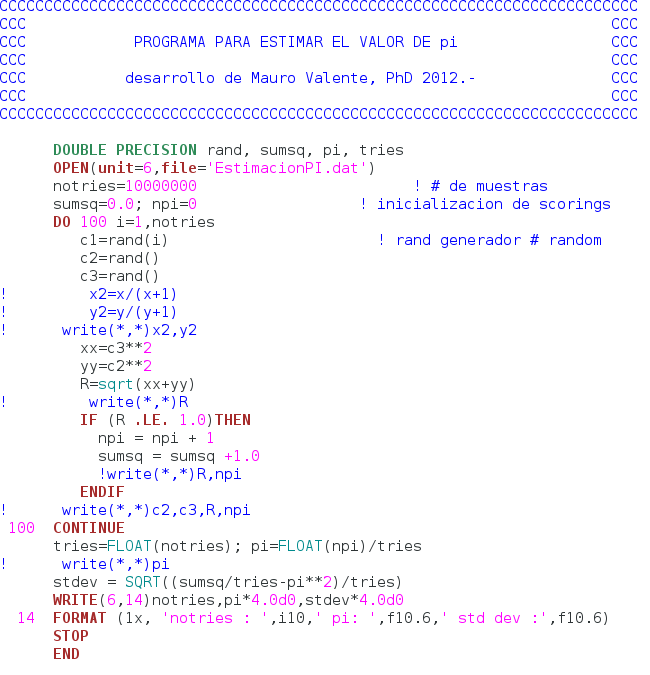
\includegraphics[width=12cm]{Figuras/Fig7_1.png}
   
\caption{Ejemplo sencillo de implementaci\'on en c\'odigo para estimaci\'on del n\'umero $\pi$ con t\'ecnica Monte Carlo.}
\label{Fig7_1}

\end{figure}
\end{center}




\section{Ejemplos de c\'alculo de integrales definidas por medio del m\'etodo Monte Carlo}
% \markboth{Intr. proc. im\'agenes radiol\'ogicas \'ambito m\'edico \ \textbf{M\'ODULO VII}}{ESPECIALIDAD III \ \textbf{M\'ODULO VII}}
\label{CapVII_4}

Se considera diferentes procedimientos para calcular integrales definidas por medio del m\'etodo Monte Carlo. 
%
El primero se llama ``M\'etodo Monte Carlo de \'exito-fracaso'', basado en la interpretaci\'on de una integral como un \'area. 
%
El segundo se llama ``m\'etodo Monte Carlo de la media muestral'' y est\'a basado en la definici\'on de valor medio de una variable 
aleatoria continua.
%

\subsection{M\'etodo de \'exito-fracaso con t\'ecnica Monte Carlo}
% \markboth{Intr. proc. im\'agenes radiol\'ogicas \'ambito m\'edico \ \textbf{M\'ODULO VII}}{ESPECIALIDAD III \ \textbf{M\'ODULO VII}}
\label{CapVII_5}

Consid\'erese el problema de calcular una integral unidimensional, donde se asume que el integrando $g(x)$ es una funci\'on acotada:

\begin{eqnarray}
 	0 \le g(x) \le c \, \; \, \; \forall x \in [a, b] \nonumber
 \label{EqZZZ12} 
\end{eqnarray}


Y sea $\Omega$ el rect\'angulo:

\begin{eqnarray}
 	\Omega = \{ (x, y) \in \Re ^{2} | \: x \in [a, b] \; y \in [0, c] \} \nonumber
 \label{EqZZZ13} 
\end{eqnarray}


Y sea $(X, Y)$ una variable aleatoria uniformemente distribuida sobre $\Omega$ con funci\'on de densidad:

\begin{eqnarray}
 	f_{x \, y} (x, y) =   \left[ \begin{array}{c}
                            \frac{1}{c} \, (b -a) \: \: (x, y) \in \Omega  \\ 
 	                    0 \: \: (x, y) \notin \Omega  \nonumber
                            \end{array} \right]
 \label{EqZZZ14} 
\end{eqnarray}


\subsection{M\'etodo de la media muestral con t\'ecnica Monte Carlo}
% \markboth{Intr. proc. im\'agenes radiol\'ogicas \'ambito m\'edico \ \textbf{M\'ODULO VII}}{ESPECIALIDAD III \ \textbf{M\'ODULO VII}}
\label{CapVII_6}

Otra forma de calcular la integral, es representarla como el valor esperado de una variable aleatoria. 
%
Se reescribe la integral definida $I$ en la forma:

\begin{eqnarray}
 	I = \int _{a} ^{b} \frac{g(x)}{f(x)} \, f(x) \: dx
 \label{EqZZZ15} 
\end{eqnarray}

Donde $f(x)$ una funci\'on de densidad correspondiente a la variable aleatoria $x$.
%

Entonces:

\begin{eqnarray}
 	I = \langle \frac{g(x)}{f(x)} \rangle
 \label{EqZZZ16} 
\end{eqnarray}

Suponiendo que la variable aleatoria se distribuye seg\'un la siguiente funci\'on de densidad:

\begin{eqnarray}
 	f(x) =  \left[  \begin{array}{c} 
               \frac{1}{(b -a)} \: \: x \in [a, b]  \\ 
 	       0 \: \: x \notin [a, b]  \end{array} \right] \nonumber
 \label{EqZZZ17} 
\end{eqnarray}


donde $x$ uniformemente distribuida en [a, b].

Entonces:

\begin{eqnarray}
 	I =  \int _{a} ^{b} g(x) \: d x = \int _{a} ^{b} \frac{1}{b -a} \, g(x) \, (b -a) \: d x =  (b - a) \langle g(x) \rangle
 \label{EqZZZ18} 
\end{eqnarray}

Por lo tanto, una estimaci\'on muestral de $I$ es:

\begin{eqnarray}
 	I \approx (b - a) \frac{1}{N} \sum _{i=1} ^{N} g(x_{i})
 \label{EqZZZ19} 
\end{eqnarray}


Mientras que el estimador para la varianza $\sigma ^{2}$ es:

\begin{eqnarray}
 	\sigma ^{2} [I] \approx \frac{1}{N - 1} \left[ \frac{\sum_{i=1} ^{N} (g(x_{i}))^{2}} {N} 
 	                                               - \left(\frac{\sum_{i=1} ^{N} g(x_{i})} {N}\right) ^{2} \right]
 \label{EqZZZ20} 
\end{eqnarray}


\subsection{Evaluaci\'on de integrales definidas}
% \markboth{Intr. proc. im\'agenes radiol\'ogicas \'ambito m\'edico \ \textbf{M\'ODULO VII}}{ESPECIALIDAD III \ \textbf{M\'ODULO VII}}
\label{CapVII_7}

A modo de ejemplo, puede calcularse $ I = \int _{0} ^{5} \frac{dx}{1 + x^{2}}$.
%

Para ello, se recurre, por ejemplo, al m\'etodo de muestreo seg\'un la expresi\'on \ref{EqZZZ19}, por lo tanto:

\begin{eqnarray}
 	I = \int _{0} ^{5} \frac{dx}{1 + x^{2}} \approx \frac{(5 - 0)}{N} \, \sum _{i=1} ^{N} \frac{1}{ 1 + (x_{i})^{2}}
 \label{EqZZZ21} 
\end{eqnarray}

A continuaci\'on, en la figura \ref{Fig7_2}, se muestra una propuesta\footnote{El c\'odigo es s\'olo para prop\'ositos ilustrativos. No se encuentra preparado de modo 
eficiente ni optimizado.} para un c\'odigo de c\'omputo para evaluar la integral $ I = \int _{0} ^{5} \frac{dx}{1 + x^{2}}$:


\begin{center}
\begin{figure} [!h]

\centering
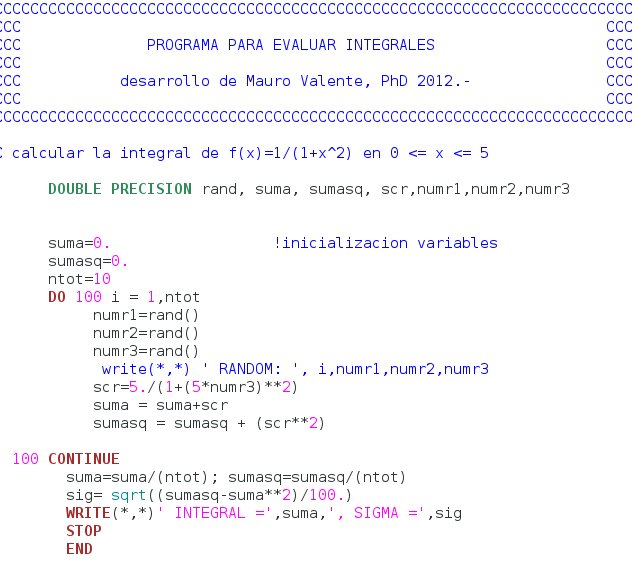
\includegraphics[width=10cm]{Figuras/Fig7_2.png}
   
\caption{Ejemplo sencillo de implementaci\'on en c\'odigo para estimaci\'on de la integral definida $ I = \int _{0} ^{5} \frac{dx}{1 + x^{2}}$ 
con t\'ecnica Monte Carlo.}
\label{Fig7_2}

\end{figure}
\end{center}

\section{El m\'etodo Monte Carlo aplicado al transporte de radiaci\'on}
% \markboth{Intr. proc. im\'agenes radiol\'ogicas \'ambito m\'edico \ \textbf{M\'ODULO VII}}{ESPECIALIDAD III \ \textbf{M\'ODULO VII}}
\label{CapVII_9}

En la actualidad, pr\'acticamente todas las \'areas recurren al uso de computadores para resolver problemas importantes,
tanto de \'indole social, econ\'omica, de ingenier\'ia, de ciencia b\'asica, aplicada, etc. 
%
Con un manejo adecuado de programas de c\'omputo e informaci\'on pueden realizarse c\'alculos y simulaciones de modelos reales,
para estudiarlos y resolver problemas te\'oricos o de aplicaci\'on.
%
Los procesos que contienen variables aleatorias son susceptibles de abordarse con el m\'etodo Monte Carlo, que siendo m\'etodo 
num\'erico capaz de explotar la capacidad de los procesadores en computadores, puede aplicarse en muchas tareas m\'as de lo que se 
hac\'ia en los principios de su aplicaci\'on pr\'actica (a principios de la d\'ecada de 1950). \\
%
%
La simulaci\'on Monte Carlo es la mejor alternativa disponible en la actualidad para resolver el problema del transporte de la 
radiaci\'on en la materia cuando se trata con geometr\'ias complejas, tales como las que se encuentran en las diversas aplicaciones
m\'edicas que utilizan radiaciones ionizantes. \\
%
%
En esta secci\'on se aborda la aplicaci\'on del m\'etodo Monte Carlo espec\'ificamente en la simulaci\'on de la interacci\'on de
la radiaci\'on con la materia, para investigar aspectos dosim\'etricos y de radiodiagn\'ostico, de algunos problemas que existen en el
\'area de f\'isica m\'edica. \\
%
%
En t\'erminos gen\'ericos, puede decirse que la simulaci\'on es un experimento te\'orico en el que se reproduce el comportamiento de
un sistema complejo, que consiste de una forma de ``realizar'' un experimento en el cual la realidad es sustituida por un modelo 
matem\'atico.\\ 
%
%
Puede considerarse como un h\'ibrido entre experimentaci\'on pura y te\'orica y es una herramienta muy \'util en la investigaci\'on 
cient\'ifica.
%
En definitiva, lo que se hacen los m\'etodos de simulaci\'on Monte Carrlo aplicados al transporte de radiaci\'on es resolver la ecuaci\'on 
de transporte de las part\'iculas de una forma puramente estad\'istica, lo cual representa ventaja sobre los m\'etodos anal\'iticos 
complejos que resuelven la ecuaci\'on de forma aproximada y s\'olo para problemas sencillos. \\
%
%
La simulaci\'on Monte Carlo en f\'isica m\'edica se utiliza para resolver problemas diversos, como estudiar y reconstruir im\'agenes de 
pacientes tomadas con equipos digitales, realizar c\'alculos de carcinog\'enesis, obtener espectros de salida de unidades de terapia, 
caracterizar detectores de radiaci\'on  y fuentes de radiaci\'on ionizante de todo tipo. \\




\subsection{Tracking de part\'iculas con el m\'etodo Monte Carlo}
% \markboth{Intr. proc. im\'agenes radiol\'ogicas \'ambito m\'edico \ \textbf{M\'ODULO VII}}{ESPECIALIDAD III \ \textbf{M\'ODULO VII}}
\label{CapVII_10}

La historia o trayectoria de una part\'icula es vista como una secuencia aleatoria de desplazamientos libres que terminan con un evento 
de interacci\'on donde la part\'icula cambia su direcci\'on de movimiento, evenbtualmente modifica el estado de fase (pierde energ\'ia o 
cambia direcci\'on de movimiento, por ejemplo) y puede generar part\'iculas secundarias. 
%
Todo ello se realiza aplicando las leyes de la f\'isica, atendiendo las funciones de probabilidad determinadas por las secciones eficaces 
adecuadas y dependiendo del medio, la energ\'ia de la part\'icula y la disposici\'on geom\'etrica del sistema. \\
%
%
A modo de ejemplo, se pueden simular condiciones extremas de un reactor nuclear, sin hacerlo en una instalaci\'on real; o bien simular la 
aplicaci\'on de un tratamiento de radioterapia a un paciente, sin llevarlo a cabo hasta que se obtengan las dosis adecuadas en los sitios 
convenientes en el simulador. \\
%
%
Se han desarrollado varios c\'odigos de simulaci\'on Monte Carlo del transporte de radiaci\'on que contienen modelos de interacci\'on para 
definir las funciones de distribuci\'on de probabilidad para las distintas variables aleatorias que intervienen en cada proceso o suceso, 
y que permiten obtener valores medios de observables de inter\'es como pueden ser la posici\'on de las part\'iculas despu\'es de cada 
interacci\'on, el momento y p\'erdidas de energ\'ia de las part\'iculas primarias o las secundarias generadas en algunas interacciones. \\
%
%
En forma gen\'erica, el objetivo de los c\'odigos de simulaci\'on es modelar el camino seguido por part\'iculas que atraviesan medios 
materiales, atendiendo las leyes de la f\'isica y las probabilidades, a partir de ciertas condiciones iniciales del estado de fase.
%
El medio en el que se lleve a cabo la simulaci\'on puede ser de estado s\'olido (generalmente amorfo), l\'iquido o gaseoso y el modelo 
geom\'etrico del sistema se define utilizando la geometr\'ia anal\'itica. \\
%
%
Los c\'odigos Monte Carlo de transporte tienen modelos de interacci\'on para las part\'iculas que se van a simular, es decir, conjuntos de 
secciones diferenciales transversales para los mecanismos de interacci\'on relevantes.
%
Se definen funciones de distribuci\'on de probabilidad para el camino libre entre interacciones, el tipo de interacci\'on que ocurre y 
el cambio del estado de fase, como p\'erdida de energ\'ia y deflexi\'on angular de las part\'iculas. \\
%
%
Algunos de los c\'odigos de simulaci\'on Monte Carlo m\'as reconocidos para el transporte de part\'iculas en medios
materiales son EGS4, EGSnrc, PENELOPE, NOREC, MCNP, GEANT4 y FLUKA. 
%
Cada c\'odigo tiene sus particularidades puede resultar m\'as conveniente para aplicaciones distintas, por lo que se debe analizar
cu\'al es el m\'as adecuado al tipo de problema, escogiendo el m\'as sencillo de acuerdo con las habilidades y capacidad de c\'omputo 
con que se cuente, y que contenga las secciones eficaces o teor\'ias f\'isicas de respaldo m\'as modernas para el tipo de part\'icula a 
simular. \\
%
%
Para varias aplicaciones en radiodiagn\'ostico y radioterapia, la utilizaci\'on de simulaci\'on Monte Carlo del transporte de la 
radiaci\'on resulta fundamentale incluso necesaria. \\
%
%
Para ejemplificar, en el caso de aplicaciones en radiodiagn\'ostico, cuando un fot\'on o un electr\'on de energ\'ia elevada penetra en un 
medio material origina una cascada de part\'iculas secundarias, cuyo n\'umero va en aumento al mismo tiempo que su energ\'ia media 
decrece. 
%
El inicio de las simulaciones de estas cascadas electromagn\'eticas, inicia con el trabajo de Berger en 1963, quien estableci\'o las
bases para realizar estos c\'alculos de forma efectiva y sobre las que todav\'ia se trabaja hoy en d\'ia. 
%
Durante las d\'ecadas de 1970 y 1980 aparecieron los primeros programas de prop\'osito general capaces de simular el transporte acoplado de 
fotones y electrones. 
%

\begin{center}
\underline{Generaci\'on de trayectorias}
\end{center}

El proceso de simulaci\'on asume que las part\'iculas siguen trayectorias rectil\'ineas a velocidad constante entre dos interacciones 
sucesivas con el medio. El modelado de su ``vida'' puede representarse como una sucesi\'on de estados determinados por la posici\'on del 
n-\'esimo suceso en la posici\'on $\vec{r}_{n}$, la direcci\'on de movimiento $\vec{\Omega}_{n}$ y energ\'ia $E_{n}$ inmediatamente 
despu\'es de producirse dicho suceso. \\
%
%
Dada una posici\'on inicial, el primer punto a resolver es determinar a qu\'e distancia se producir\'a el siguiente suceso y, luego, de qu\'e 
tipo ser\'a. 
%
La primera cuesti\'on se resuelve teniendo en cuenta el hecho de que el viaje de una part\'icula constituye un proceso de Poisson; la 
segunda, considerando la relaci\'on entre las secciones eficaces de las diversas interacciones posibles. \\
%
%
Si $\lambda_{i}$ representa el recorrido libre medio (mfp) correspondiente a la interacci\'on de tipo ``i'', y $\lambda$ el mfp total (cuyo 
inverso es la suma de inversos de los recorridos libres medios parciales), la distancia $s$ recorrida por la part\'icula hasta el pr\'oximo 
suceso se determina mediante la expresi\'on \ref{EqZZZ22}:

\begin{eqnarray}
 	s = -\lambda \, \ln (\zeta)
 \label{EqZZZ22} 
\end{eqnarray}

donde $\zeta$ es un n\'umero aleatorio uniformemente en [0, 1].  \\
%
%
La probabilidad $P_{i}$ de que la interacci\'on sea del i-\'esimo tipo es:

\begin{eqnarray}
 	P_{i} = \frac{\lambda}{\lambda_{i}}
 \label{EqZZZ23} 
\end{eqnarray}

Una vez sorteado el tipo de interacci\'on a simular de acuerdo con las probabilidades expresadas por en la ecuaci\'on \ref{EqZZZ23}, es 
necesario simular el cambio de estado (t\'ipicamente direcci\'on y energ\'ia) que haya podido producirse. 
%
Para ello se emplea la distribuci\'on de probabilidad asociada a la secci\'on eficaz doble diferencial correspondiente. \\
%
%
Por tanto, el proceso transforma el estado $(\vec{r}_{n}, \vec{\Omega}_{n}, E_{n})$ al $(\vec{r}_{n+1}, \vec{\Omega}_{n+1}, E_{n+1})$. 
%
El proceso se repite hasta que, o bien la part\'icula escapa del sistema material, o bien su energ\'ia cae por debajo de cierto valor, 
momento en el cual se supone que es localmente absorbida y su vida terminada. 
%
Tras simular la vida de una part\'icula debe hacerse lo propio con las part\'iculas secundarias a las que haya dado lugar. \\
%
%
\subsection{Modelado de colisiones e interacciones con el m\'etodo Monte Carlo}
% \markboth{Intr. proc. im\'agenes radiol\'ogicas \'ambito m\'edico \ \textbf{M\'ODULO VII}}{ESPECIALIDAD III \ \textbf{M\'ODULO VII}}
\label{CapVII_11}

Los procesos de colisi\'on se implementan en la t\'ecnica de simulaci\'on Monte Carlo por medio de modelos de interacci\'on que determinan 
las secciones eficaces.
%
Para ello, en las aplicacionmes t\'ipicas de transporte de radiaci\'on ionizante, se requiere el conocimiento de las secciones eficaces 
doble diferencial en energ\'ia y \'angulo s\'olido. 
%
Los valores de las secciones eficaces pueden ser introducidos en la simulaci\'on Monte Carlo por medio de modelos an\'aliticos que son 
directamente evaluados para las variables de estado de cada caso; y tambi\'en puede emplearse tablas de valores obtenidas de bases de 
datos, que requieren procesos posteriores para interpolar (asumiendo continuidad) permitiendo obtener el valor correspondiente a las 
variables de estado. \\
%
%
\begin{center}
\underline{T\'ecnicas de simulaci\'on condensada}
\end{center}

En principio, el esquema de simulaci\'on anteriormente presentado es v\'alido para cualquier tipo de part\'icula. 
%
En la pr\'actica, sin embargo, no resulta adecuado cuando se consideran -por ejemplo- electrones de alta energ\'ia, dado que el n\'umero 
de interacciones a lo largo de su trayectoria antes de ser absorbidos resulta excesivamente elevado, del orden de algunas decenas de 
miles para electrones de 1 MeV, por ejemplo. 
%
Tal cantidad de colisiones requerir\'ia un tiempo de simulaci\'on tan grande que convierte a la soluci\'on propuesta al problema en algo 
inviable. \\
%
%
El modo de resolver las dificultades derivadas de este inconveniente se recurre a una t\'ecnica denominada ``simulaci\'on condensada'', 
cuyo fundamento se encuentra en las teor\'ias de dispersi\'on m\'ultiple. 
%
La idea consiste, b\'asicamente, en simular el efecto global neto de un n\'umero elevado de interacciones mediante un \'unico suceso 
``artificial''. 
%
Exista una variante, propuesta por Berger, conocida como simulaci\'on mixta, que se combina la simulaci\'on detallada de los sucesos m\'as 
``violentos'' con la condensada de los restantes, resultando un algoritmo particularmente robusto y vers\'atil. \\
%
%
Los diversos esquemas de simulaci\'on condensada constituyen quiz\'as la principal caracter\'istica que distingue los programas de uso 
m\'as extendido. 
%
De hecho, la concepci\'on de nuevos algoritmos m\'as precisos y m\'as r\'apidos es uno de los temas de investigaci\'on abiertos en el 
campo de la simulaci\'on Monte Carlo del transporte de la radiaci\'on. \\
%
%
\vspace{1.0cm}

\begin{center}
\underline{Cantidades de inter\'es en la simulaci\'on de part\'iculas}
\end{center}

Para obtener el valor medio de un observable $Q$ ($ \langle Q \rangle $) por medio de simulaci\'on Monte Carlo, en el transporte de 
radiaci\'on, conviene introducir el concepto de ``historia'' entendida como la ``vida'' de una part\'icula primaria y la de todas las 
secundarias generadas por \'esta. 
%
A modo de ejemplo, podr\'ia tratarse de la dosis en un cierto volumen de inter\'es. \\
%
%
Sea $q_{j}$ a la contribuci\'on de la j-\'esima historia, la estimaci\'on del valor medio del observable (en el ejemplo, la energ\'ia 
depositada por historia) tras simular un total de $N$ historias prove\'e el siguiente estimador para $q$ para $\langle Q \rangle$:

\begin{eqnarray}
 	\langle Q \rangle \sim q \equiv \frac{1}{N} \sum_{j=1} ^{N} q_{j}
 \label{EqZZZ24} 
\end{eqnarray}

que coincide con la expresi\'on \ref{EqZZZ1}. \\
%
%


\subsection{Ejemplo b\'asico artificial de transporte con el m\'etodo Monte Carlo}
% \markboth{Intr. proc. im\'agenes radiol\'ogicas \'ambito m\'edico \ \textbf{M\'ODULO VII}}{ESPECIALIDAD III \ \textbf{M\'ODULO VII}}
\label{CapVII_12}


A modo de ejemplo extremamente sencillo, se propone realizar el modelado por simulaci\'on Monte Carlo de una part\'icula libre movi\'endose
en un plano. 
%
El problema conocido como \textit{random walk} consiste en mover una part\'icula con paso $p$ con caracter\'isticas isotr\'opicas y 
homog\'eneas para el medio en que se transporta la part\'icula. \\
%
%
Entonces, la distribuci\'on angular que corresponde al cambio en la direcci\'on de movimiento es isotr\'opica, y se busca, en general,
determinar la distancia neta recorrida al cabo de $N$ movimientos. \\
%
%

\subsection{Ejemplo sencillo de transporte con el m\'etodo Monte Carlo: Columna de neutrones}
% \markboth{Intr. proc. im\'agenes radiol\'ogicas \'ambito m\'edico \ \textbf{M\'ODULO VII}}{ESPECIALIDAD III \ \textbf{M\'ODULO VII}}
\label{CapVII_13}

El transporte de neutrones, por ejemplo, puede implementarse siguiendo, a grandes l\'ineas seg\'un el esquema:

\begin{enumerate}
 \item Definici\'on de la geometr\'ia del problema.
 \item Definici\'on de la fuente.
 \item Selecci\'on del tipo de part\'icula para la fuente.
 \item Determinaci\'on de la posici\'on de colisi\'on.
 \item Determinaci\'on del tipo de interacci\'on.
 \item Determinaci\'on del resultado de la interacci\'on.
 \item Finalizaci\'on de la historia de los secundarios.
 \item C\'alculo de los estimadores.
\end{enumerate}

A modo de ejemplo, se considera una fuente puntual que emite un pulso, es decir una funci\'on $\delta$, neutrones en la direcci\'on $z$ y
est\'a inmersa en un medio material homog\'eneo e isotr\'opico. Se considera como geometr\'ia una esfera de radio $R$ y ausencia de 
absorci\'on y el movimiento de las part\'iculas es siempre en direcci\'on $z$ alej\'andose de la fuente. Estimar
la cantidad de interacciones que ocurren dentro de la geometr\'ia, introduciendo el modelado y par\'ametros que sean necesarios.